\documentclass{article}
\usepackage{iclr2025_conference,times}
\input{math_commands.tex}

\usepackage{hyperref}
\usepackage{url}
\usepackage{graphicx}
\usepackage{booktabs}
\usepackage{tabularx}
\usepackage{array}
\usepackage{float}

\title{Detecting LLM-Generated Student Essays with Transformer Fine-Tuning and Robustness Analysis}

\author{Joseph Souaiby - Huzaifah Wasim}

\iclrfinalcopy
\begin{document}

\maketitle

\begin{figure}[H]
\centering

\includegraphics[width=0.9\linewidth]{figures/teaser.png}
\caption{Teaser figure summarizing the current milestone pipeline and the remaining transformer stage.}
\label{fig:teaser}
\end{figure}

\section{Introduction}
Large language models now produce fluent long-form writing that is increasingly difficult to distinguish from human-authored essays, which creates obvious risks for academic integrity, misuse, and unreliable automated moderation. Our project studies AI-text detection in a realistic setting: binary classification of full essays as either human-written or machine-generated, with an emphasis on whether detectors generalize beyond a single benchmark.

The input to our system is raw essay text, and the output is a probability that the essay was AI-generated. At this milestone stage, training is supervised on the Kaggle \emph{LLM Detect AI Generated Text} dataset \citep{thite2026kaggle}, while robustness is evaluated out of domain on RAID \citep{dugan2024raid}. We treat the problem as essay-level binary classification and use held-out evaluation plus cross-dataset transfer to distinguish in-domain fitting from genuine generalization.

Our current milestone goals are: (1) establish strong classical baselines, (2) quantify how much performance degrades under dataset shift, and (3) prepare the full transformer training pipeline for the final phase. The results already show a useful tension: sparse lexical baselines achieve nearly perfect in-domain performance, but they fail badly out of domain, which suggests benchmark-specific artifacts rather than robust detection. This directly motivates the next-stage transformer model and ablation plan.
The public project repository is available at \url{https://github.com/Joseph-Souaiby/DeepLearningProject.git}.

\section{Related Work}
AI-text detection has been approached from both likelihood-based heuristics and supervised representation learning. GLTR \citep{gehrmann2019gltr} shows that token-rank statistics from a language model can expose generation artifacts, while DetectGPT \citep{mitchell2023detectgpt} proposes a training-free signal based on curvature of log-likelihood under perturbations. These works motivate our GLTR-style baseline because they capture generation regularities without relying on sparse word overlap alone.

For supervised detection, transformer encoders such as BERT \citep{devlin2019bert} and RoBERTa \citep{liu2019roberta} provide strong contextual representations for document classification, and they are natural candidates for our main model. Their success, however, does not automatically imply robustness to generator or domain shift. Benchmark papers such as TURINGBENCH \citep{uchendu2021turingbench} and HC3 \citep{guo2023hc3} show that detector transfer across domains and generators remains difficult, which is why our milestone explicitly measures out-of-domain (OOD) transfer.

Our data choice also follows this literature. We train on the Kaggle student-essay dataset \citep{thite2026kaggle}, because it matches the educational writing setting we care about, and we evaluate OOD on RAID \citep{dugan2024raid}, which provides a distribution shift in both topic and generation conditions. For the final stage, we also plan parameter-efficient fine-tuning via LoRA \citep{hu2022lora} so that we can run more robustness sweeps under limited compute.

\section{Problem Decomposition \& Detailed Technical Approach}
\paragraph{Problem formulation.}
We learn a detector $f(x) \rightarrow [0,1]$ that maps an essay $x$ to the probability that it is AI-generated. The main supervised training corpus is the Kaggle dataset. After whitespace normalization, duplicate removal, and a minimum-length filter, the dataset contains 27{,}278 essays. We use stratified train/validation/test splits of 21{,}822 / 2{,}728 / 2{,}728 essays. For OOD evaluation, we stream RAID from Hugging Face and sample 10{,}000 examples with the original class proportions preserved (5{,}900 human, 4{,}100 AI).

\paragraph{Current baselines.}
Our first baseline family uses TF-IDF features with up to 50{,}000 unigram and bigram features, sublinear term frequency, and standard document-frequency filtering. We train two linear classifiers on the same features: logistic regression and linear SVM.

Our second baseline family is a GLTR-style likelihood heuristic inspired by \citet{gehrmann2019gltr}. We score each essay with a small causal language model (DistilGPT-2) and aggregate 16 essay-level statistics, including mean token log-probability, surprisal, entropy, average rank, rank variance, and the fraction of tokens in the top-10/top-100/top-1000 predictions. These dense features are standardized and fed into the same logistic regression and linear SVM classifiers. This keeps the evaluation protocol parallel to TF-IDF while testing a more generation-aware signal.

\paragraph{Primary deep model for the final phase.}
Our planned main method is transformer fine-tuning with BERT or RoBERTa \citep{devlin2019bert,liu2019roberta}. Essays will be tokenized and truncated to a fixed maximum length, encoded with a pre-trained transformer, and classified through a task-specific linear head. We will optimize cross-entropy with class balancing and early stopping on validation macro-F1/AUROC. We also plan a LoRA variant \citep{hu2022lora} to compare full fine-tuning against a cheaper adaptation strategy.

\paragraph{Research hypotheses (CS7643).}
\textbf{H1:} A fine-tuned transformer encoder will outperform both TF-IDF and GLTR baselines on Kaggle in macro-F1 and AUROC under the same train/validation/test split.\\
\textbf{H2:} A transformer trained with artifact-aware preprocessing (duplicate removal, whitespace normalization, and prompt-format normalization) will exhibit a smaller Kaggle-to-RAID macro-F1 drop than the same architecture trained on minimally processed text.\\
\textbf{H3:} LoRA fine-tuning will match full fine-tuning within 2 macro-F1 points on Kaggle while reducing trainable parameters enough to enable broader OOD ablations.

\paragraph{Evaluation protocol.}
All baselines and future transformer models will use the same splits and evaluation procedure. We report accuracy, macro-F1, class-wise precision/recall, AUROC plots, and confusion matrices. Final success is not just high Kaggle accuracy; it also requires materially better OOD behavior on RAID than our current sparse baselines. This evaluation directly tests whether a detector has learned robust writing signals rather than dataset-specific shortcuts.

\section{Experiments \& Results}
\paragraph{Dataset inspection.}
We began with exploratory analysis on the Kaggle corpus to understand label balance and stylistic differences before training. Figure~\ref{fig:eda} shows two examples from the current analysis notebook: the class distribution and a length-based comparison. These diagnostics helped justify both baseline families: TF-IDF can exploit lexical and formatting cues, while GLTR-style features may capture differences in essay predictability under a language model.

\begin{figure}[t]
\centering
\begin{minipage}[t]{0.47\linewidth}
\centering

\includegraphics[width=\linewidth]{figures/kaggle_class_distribution.png}
\end{minipage}
\hfill
\begin{minipage}[t]{0.47\linewidth}
\centering

\includegraphics[width=\linewidth]{figures/kaggle_length_analysis_03.png}
\end{minipage}
\caption{Two representative exploratory plots from the current baseline pipeline: class balance (left) and length metrics by class (right).}
\label{fig:eda}
\end{figure}

\paragraph{Baseline results.}
Table~\ref{tab:main-results} summarizes the four current baselines. TF-IDF performs extremely well on the Kaggle test split, reaching 99.74\% accuracy with linear SVM. However, these same models collapse on RAID, with only about 41\% accuracy and macro-F1 around 0.29. In contrast, the GLTR-style baseline is weaker in domain (95.42--95.64\% accuracy) but noticeably more robust OOD, reaching 57.78\% accuracy and 0.56 macro-F1 with logistic regression.

\begin{table}[t]
\centering
\small
\begin{tabular}{llcccc}
\toprule
Dataset & Method & Acc. & Macro-F1 & Human Recall & AI Recall \\
\midrule
Kaggle & TF-IDF + LogReg & 99.12 & 0.99 & 1.00 & 0.98 \\
Kaggle & TF-IDF + SVM & 99.74 & 1.00 & 1.00 & 0.99 \\
Kaggle & GLTR + LogReg & 95.42 & 0.95 & 0.95 & 0.96 \\
Kaggle & GLTR + SVM & 95.64 & 0.96 & 0.96 & 0.96 \\
\midrule
RAID & TF-IDF + LogReg & 40.86 & 0.29 & 0.00 & 1.00 \\
RAID & TF-IDF + SVM & 40.90 & 0.29 & 0.00 & 0.99 \\
RAID & GLTR + LogReg & 57.78 & 0.56 & 0.30 & 0.97 \\
RAID & GLTR + SVM & 55.20 & 0.52 & 0.26 & 0.97 \\
\bottomrule
\end{tabular}
\caption{Current milestone baseline results extracted from \texttt{Baselines.ipynb}. The sharp drop from Kaggle to RAID shows that in-domain benchmark accuracy alone is misleading.}
\label{tab:main-results}
\end{table}

\paragraph{Interpreting the milestone.}
The most important finding so far is not that TF-IDF is ``good,'' but that it is probably too good on Kaggle. Near-perfect in-domain scores combined with catastrophic RAID transfer strongly suggest that the model is exploiting narrow lexical or formatting artifacts. The GLTR-style baseline provides a stronger robustness reference point: it still struggles OOD, but it is substantially better than TF-IDF under shift. This makes it an appropriate baseline for the transformer phase.

\paragraph{Status of our proposed method.}
We do not yet report transformer accuracy, but implementation progress is concrete. The end-to-end data cleaning, visualization, metric generation, OOD evaluation, and likelihood-feature pipeline are complete, and the local environment is now GPU-enabled for PyTorch. The next step is to plug a BERT/RoBERTa classifier into the same evaluation harness and compare its OOD degradation against the baselines above.

\begin{figure}[t]
\centering
\begin{minipage}[t]{0.47\linewidth}
\centering
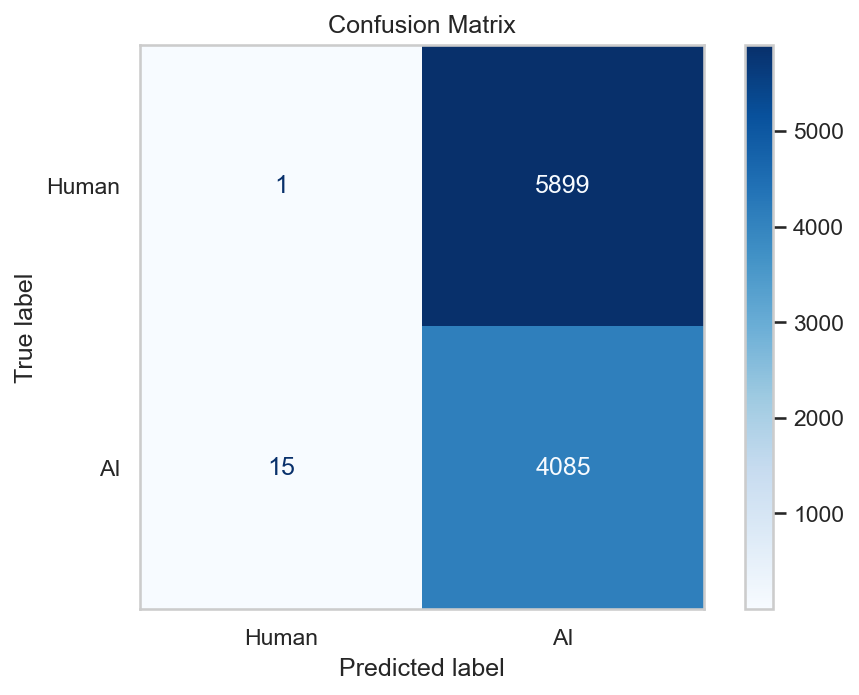
\includegraphics[width=\linewidth]{figures/raid_tfidf_logreg_cm.png}
\end{minipage}
\hfill
\begin{minipage}[t]{0.47\linewidth}
\centering
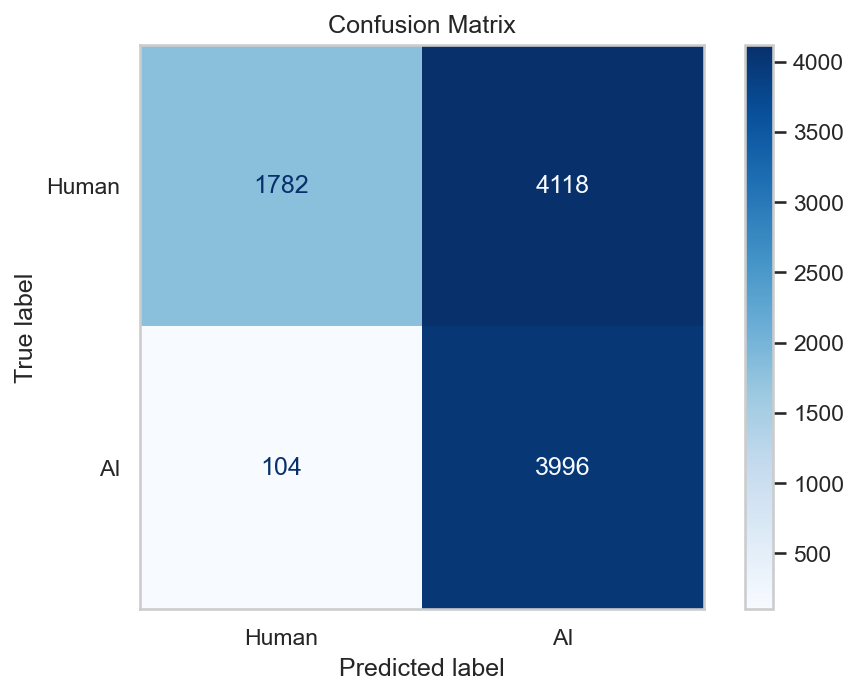
\includegraphics[width=\linewidth]{figures/raid_gltr_logreg_cm.png}
\end{minipage}
\caption{OOD confusion matrices on RAID for logistic regression. TF-IDF (left) nearly collapses to predicting the AI class, while the GLTR-style baseline (right) recovers more human examples.}
\label{fig:raid-cm}
\end{figure}

\section{Next Steps}
Our remaining plan is organized around three milestones. \textbf{First}, implement and train a RoBERTa/BERT essay classifier using the same cleaned Kaggle split, with validation-based checkpointing and full metric logging. \textbf{Second}, run the planned ablations tied to H1--H3: sequence length, artifact-aware preprocessing, and LoRA vs. full fine-tuning. \textbf{Third}, evaluate every transformer variant on RAID and compare both in-domain performance and OOD degradation against TF-IDF and GLTR baselines.

The main risks are overfitting to benchmark artifacts, essay length constraints for transformer inputs, and limited time for large hyperparameter sweeps. We will mitigate these by keeping the evaluation harness fixed, prioritizing macro-F1 and OOD transfer over raw Kaggle accuracy, using artifact normalization in preprocessing, and adopting LoRA if full fine-tuning becomes too expensive. Our success criterion for the final report is a transformer-based detector that beats the GLTR baseline on Kaggle while also improving RAID macro-F1 enough to show a clear robustness gain, rather than only a benchmark-specific boost.

\bibliography{milestone_refs}
\bibliographystyle{iclr2025_conference}

\end{document}
